%%%%%%%%%%%%%%%%%%%%%%%%%%%%%%%%%%%%%%%%%
% Arsclassica Article
% LaTeX Template
% Version 1.1 (10/6/14)
%
% This template has been downloaded from:
% http://www.LaTeXTemplates.com
%
% Original author:
% Lorenzo Pantieri (http://www.lorenzopantieri.net) with extensive modifications by:
% Vel (vel@latextemplates.com)
%
% License:
% CC BY-NC-SA 3.0 (http://creativecommons.org/licenses/by-nc-sa/3.0/)
%
%%%%%%%%%%%%%%%%%%%%%%%%%%%%%%%%%%%%%%%%%

%----------------------------------------------------------------------------------------
%	PACKAGES AND OTHER DOCUMENT CONFIGURATIONS
%----------------------------------------------------------------------------------------

\documentclass[
article,
10pt, % Main document font size
oneside, % One page layout (no page indentation)
BCOR5mm, % Binding correction
]{scrartcl}
\usepackage[a4paper,margin=3cm]{geometry}
\usepackage[italian]{babel}
\usepackage[utf8]{inputenc}
\usepackage{atbegshi}% http://ctan.org/pkg/atbegshi
\usepackage{tikz}
\usetikzlibrary{shapes}
\usepackage{amsmath}
\usepackage{xspace}
\usepackage[usestackEOL]{stackengine}
\usepackage{graphicx}
\usepackage{caption}
\usepackage{hyperref}
\usepackage{subcaption}
\usepackage{float}
\newcommand{\A}{\ensuremath{\mathcal{A}}\xspace}
\newcommand{\B}{\ensuremath{\mathcal{B}}\xspace}
\newcommand\pa[1]{\ensuremath{\left(#1\right)}}
\AtBeginDocument{\AtBeginShipoutNext{\AtBeginShipoutDiscard}}

\hyphenation{Fortran hy-phen-ation} % Specify custom hyphenation points in words with dashes where you would like hyphenation to occur, or alternatively, don't put any dashes in a word to stop hyphenation altogether

%----------------------------------------------------------------------------------------
%	TITLE AND AUTHOR(S)
%----------------------------------------------------------------------------------------

\begin{document}

\begin{center}
\title{
  \begin{figure}[h!]
  \centering
  
\includegraphics[width=.3\columnwidth]{images/logo_padova.jpg}
  \end{figure}
  Alternating Bit Protocol \\
  \vspace{2cm}
  Progetto di \textbf{Linguaggi e Modelli per il Global Computing}
}
\author{
Sebastiano Valle 1050123}
\end{center} % The article author(s) - author affiliations need to be specified in the AUTHOR AFFILIATIONS block






%\date{} % An optional date to appear under the author(s)

%----------------------------------------------------------------------------------------

%----------------------------------------------------------------------------------------
%	TABLE OF CONTENTS & LISTS OF FIGURES AND TABLES
%----------------------------------------------------------------------------------------

\maketitle % Print the title/author/date block

\setcounter{page}{1} % Set the depth of the table of contents to show sections and subsections only


\raggedright{}
\newpage{}
\tableofcontents % Print the table of contents



\listoffigures % Print the list of figures

\listoftables % Print the list of tables

\section{Introduzione}

\subsection{Funzionamento}\label{sec:intro}
ABP (\emph{Alternating Bit Protocol}) è un protocollo di rete operante al
livello data link.

Tale tecnologia si assicura che la comunicazione tra due nodi adiacenti avvenga
correttamente, adottando le seguenti regole:

\begin{itemize}
  \item I messaggi vengono spediti unidirezionalmente, dal
    trasmittente A (o \emph{Sender}) al ricevente B (o
    \emph{Receiver})\footnote{si assume che il canale di trasmissione sia di
    tipo FIFO};
  \item Ad ogni messaggio è abbinato un numero (un bit) che indica il numero di
    sequenza, 0 o 1;
  \item Ogni messaggio che A deve trasmettere ha numero di sequenza diverso dal
    messaggio successivo che deve spedire;
  \item Alla ricezione del messaggio, B può mandare ad A:
  \begin{itemize}
    \item un messaggio di conferma di corretta ricezione
      (\emph{Acknowledgement}) \texttt{ACKX}, dove X è il numero di sequenza
      del messaggio ricevuto;
    \item un messaggio di conferma di ricezione con errori
      (\emph{Negative Acknowledgement}) \texttt{NACKX}, dove X è il numero di
      sequenza del messaggio ricevuto.
  \end{itemize}
  \item I messaggi vengono trasmessi continuamente da A senza rimanere
    bloccato in attesa di una qualsiasi risposta da B;
  \item Nel caso in cui A ricevesse un \emph{acknowledgement} per il messaggio
    che sta trasmettendo, deve cominciare la trasmissione del prossimo
    messaggio;
  \item finchè A sta trasmettendo un messaggio con numero di sequenza, tutti
    gli \texttt{ACK} e i \texttt{NACK} con numero di sequenza diverso dovranno
    essere ignorati.
\end{itemize}

\begin{figure}[H]
  \centering
  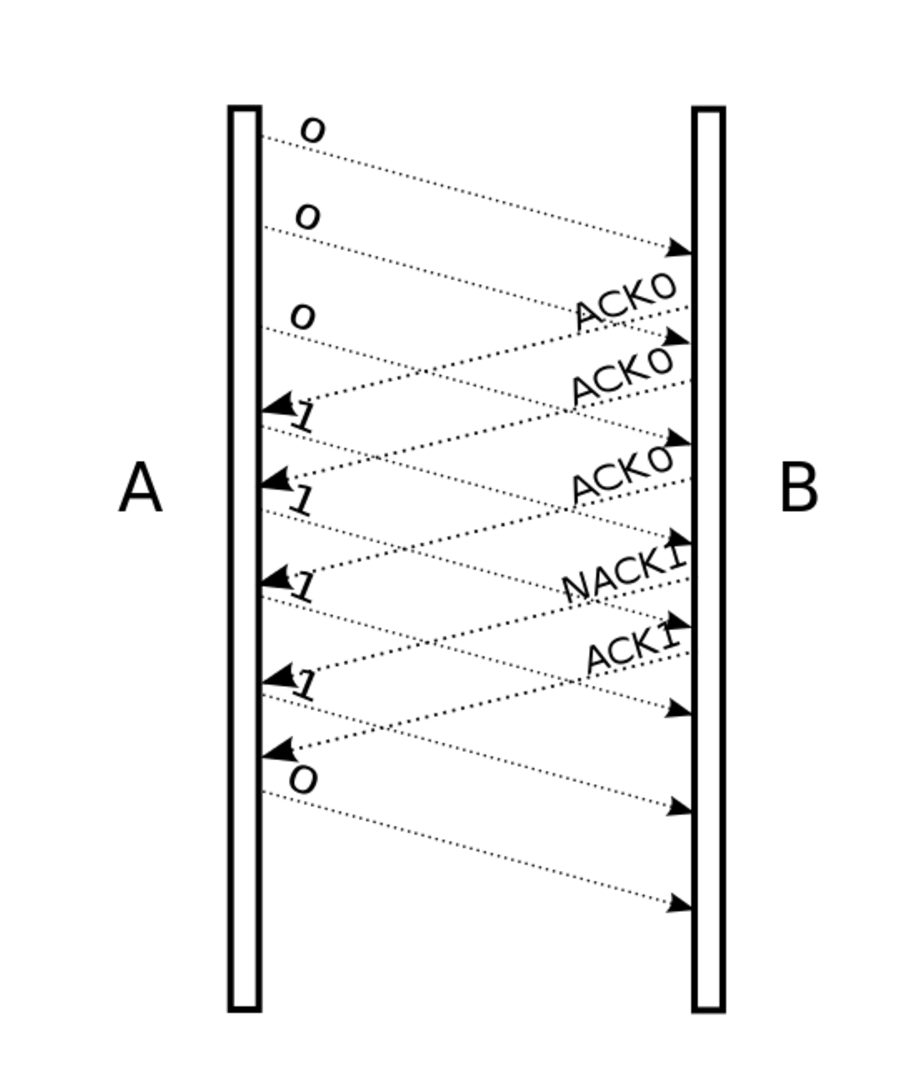
\includegraphics[width=.5\columnwidth]{images/abp.eps}
  \caption{Protocollo ABP}
  \label{fig:graphic-abp}
\end{figure}
 % 100%
\newpage{}\section{Rappresentazione con CCS}

\subsection{Modellazione tramite CCS}\label{sec:ccs-model}

In prima battuta, è doveroso modellare il protocollo con il CCS(\emph{Calculus
of Communicating Systems}).

Vengono quindi individuati i seguenti agenti:

\begin{itemize}
\item \textbf{Memory}: cella di memoria in cui è possibile leggere o scrivere
  il numero di sequenza di un messaggio;
\item \textbf{Sender}: processo che legge continuamente il numero di sequenza
  corrente dalla memoria e trasmette un messaggio con numero di sequenza
  uguale all'esito di tali letture;
\item \textbf{Receiver}: processo che riceve i messaggi spediti da
  \textbf{Sender}, fornendo sempre conferme (\texttt{ACKX});
\item \textbf{BadReceiver}: variante del Receiver, non accetta sempre i
  messaggi in ingresso (fornisce sia \texttt{ACKX} che \texttt{NACKX});
\item \textbf{AckReceiver}: processo che rimane in ascolto di comunicazioni di
  corretta o errata ricezione da parte di un \textbf{Receiver} o un
  \textbf{BadReceiver}. \\
  Nel caso in cui un messaggio accompagnato da numero di sequenza X venga
  trasmesso correttamente, \textbf{AckReceiver} cambia il valore nella cella
  di memoria.
\end{itemize}

Gli agenti sopra menzionati usano i seguenti canali (per facilità di notazione
scritti usando il VP-CCS (\emph{Value Passing-CCS}));

\begin{itemize}
\item \textbf{read(x)}: canale utilizzato per leggere lo stato della cella di
  memoria. \\
  L'argomento \texttt{x} è lo stato salvato in \textbf{Memory};
\item \textbf{write(x)}: canale utilizzato per aggiornare lo stato della cella
  di memoria. \\
  L'argomento \texttt{x} è lo stato che si vuole scrivere in \textbf{Memory};
\item \textbf{msg(x)}: canale utilizzato per mandare un messaggio da
  \textbf{Sender} a \textbf{Receiver}. \\
  Ha come argomento il numero di sequenza \texttt{x} associato al messaggio
  spedito;
\item \textbf{ack(x)}: canale utilizzato per confermare la corretta ricezione
  del messaggio avente numero di sequenza \texttt{x};
\item \textbf{nack(x)}: canale utilizzato per notificare l'errata ricezione
  del messaggio avente numero di sequenza \texttt{x};
\item \textbf{ok(x)}: canale utilizzato per notificare la corretta trasmissione
  del messaggio avente numero di sequenza \texttt{x};
\end{itemize}

Viene quindi esposto in CCS come gli agenti comunicano tra di loro affinchè i
requisiti esposti in sezione \ref{sec:intro} siano soddisfatti: \\

$ $

$ > Memory_0 := \overline{read}_0.Memory_0 + write_1.Memory_1 $

$ > Memory_1 := \overline{read}_1.Memory_1 + write_0.Memory_0 $

$ $

$ > Sender := read_0.(\overline{msg}_0.Sender + read_1.Sender) +
              read_1.(\overline{msg}_1.Sender + read_0.Sender) $

$ $

$ > Receiver_0 := msg_0.\overline{ack}_0.Receiver_1 $

$ > Receiver_1 := msg_1.\overline{ack}_1.Receiver_0 $

$ $

$ > BadReceiver_0 := msg_0.(\overline{ack}_0.BadReceiver_1 +
                            \overline{nack}_0.BadReceiver_0) $

$ > BadReceiver_1 := msg_1.(\overline{ack}_1.BadReceiver_0 +
                            \overline{nack}_1.BadReceiver_1) $

$ $

$ > AckReceiver_0 := ack_0.AckReceiver_{M0} +
                     nack_0.AckReceiver_0 + ack_1.AckReceiver_0) $

$ > AckReceiver_{M0} := \overline{write}_1.ok_0.AckReceiver_1 $

$ > AckReceiver_1 := ack_1.AckReceiver_{M1} +
                     nack_1.AckReceiver_1 + ack_0.AckReceiver_1) $

$ > AckReceiver_{M1} := \overline{write}_0.ok_1.AckReceiver_0 $

$ $

$ > Sys_{Reliable} =  (Sender | Receiver_0 | AckReceiver_0 | Memory_0) $
  \textbackslash{} $ \{msg_0,msg_1,read_0,read_1,write_0,write_1,
                       ack_0,ack_1,nack_0,nack_1\} $

$ $

$ > Sys_{Unreliable} =  (Sender | BadReceiver_0 | AckReceiver_0 | Memory_0) $
  \textbackslash{} $ \{msg_0,msg_1,read_0,read_1,write_0,write_1,
                       ack_0,ack_1,nack_0,nack_1\} $

\begin{figure}[H]
  \centering
  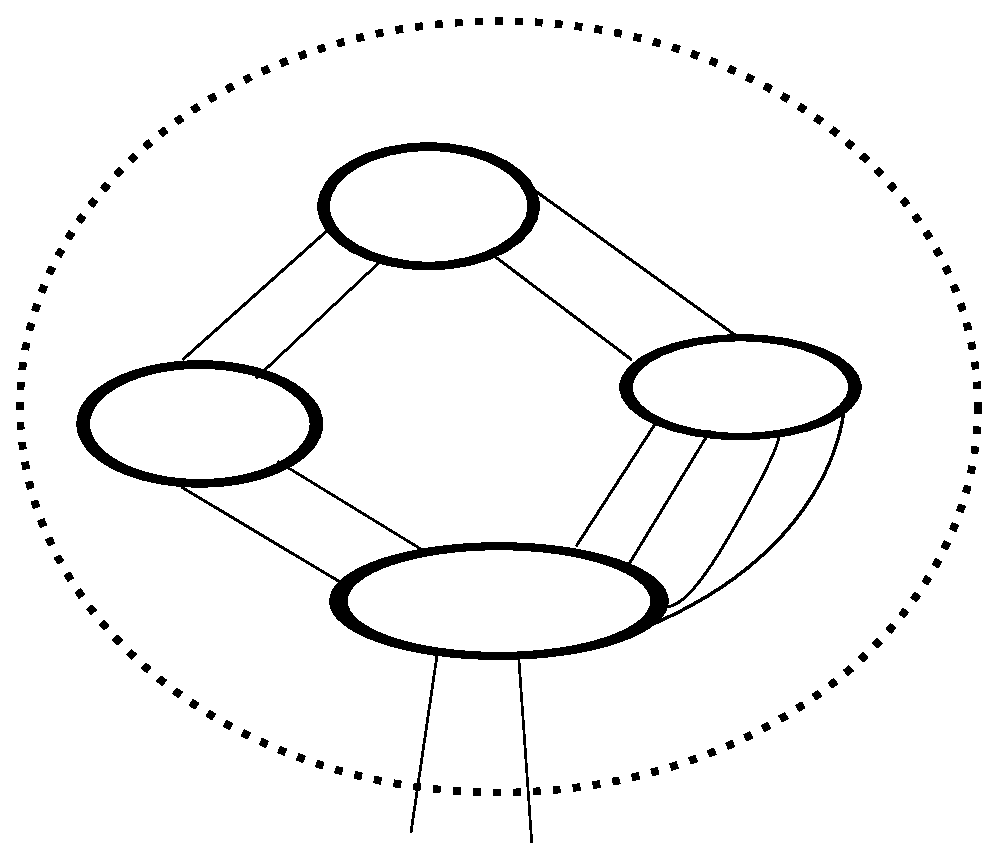
\includegraphics[width=.5\columnwidth]{images/ccs.eps}
  \caption{Rappresentazione di ABP tramite CCS}
  \label{fig:ccs-abp}
\end{figure}

\subsection{pseuCo}

Il sistema è stato provato anche su \url{pSeuco.com} (script
\ref{sec:pseuco-script}). 

Sebbene il grafico risultante è piuttosto confusionario, sembra che la
rappresentazione del sistema in CCS soddisfi le proprietà attese.

Nella parte superiore del grafico vi sono tutte le notifiche da parte di
\texttt{$AckReceiver_1$} di corretta ricezione, mentre nella parte inferiore
quelle di \texttt{$AckReceiver_0$}:

\begin{figure}[H]
  \centering
  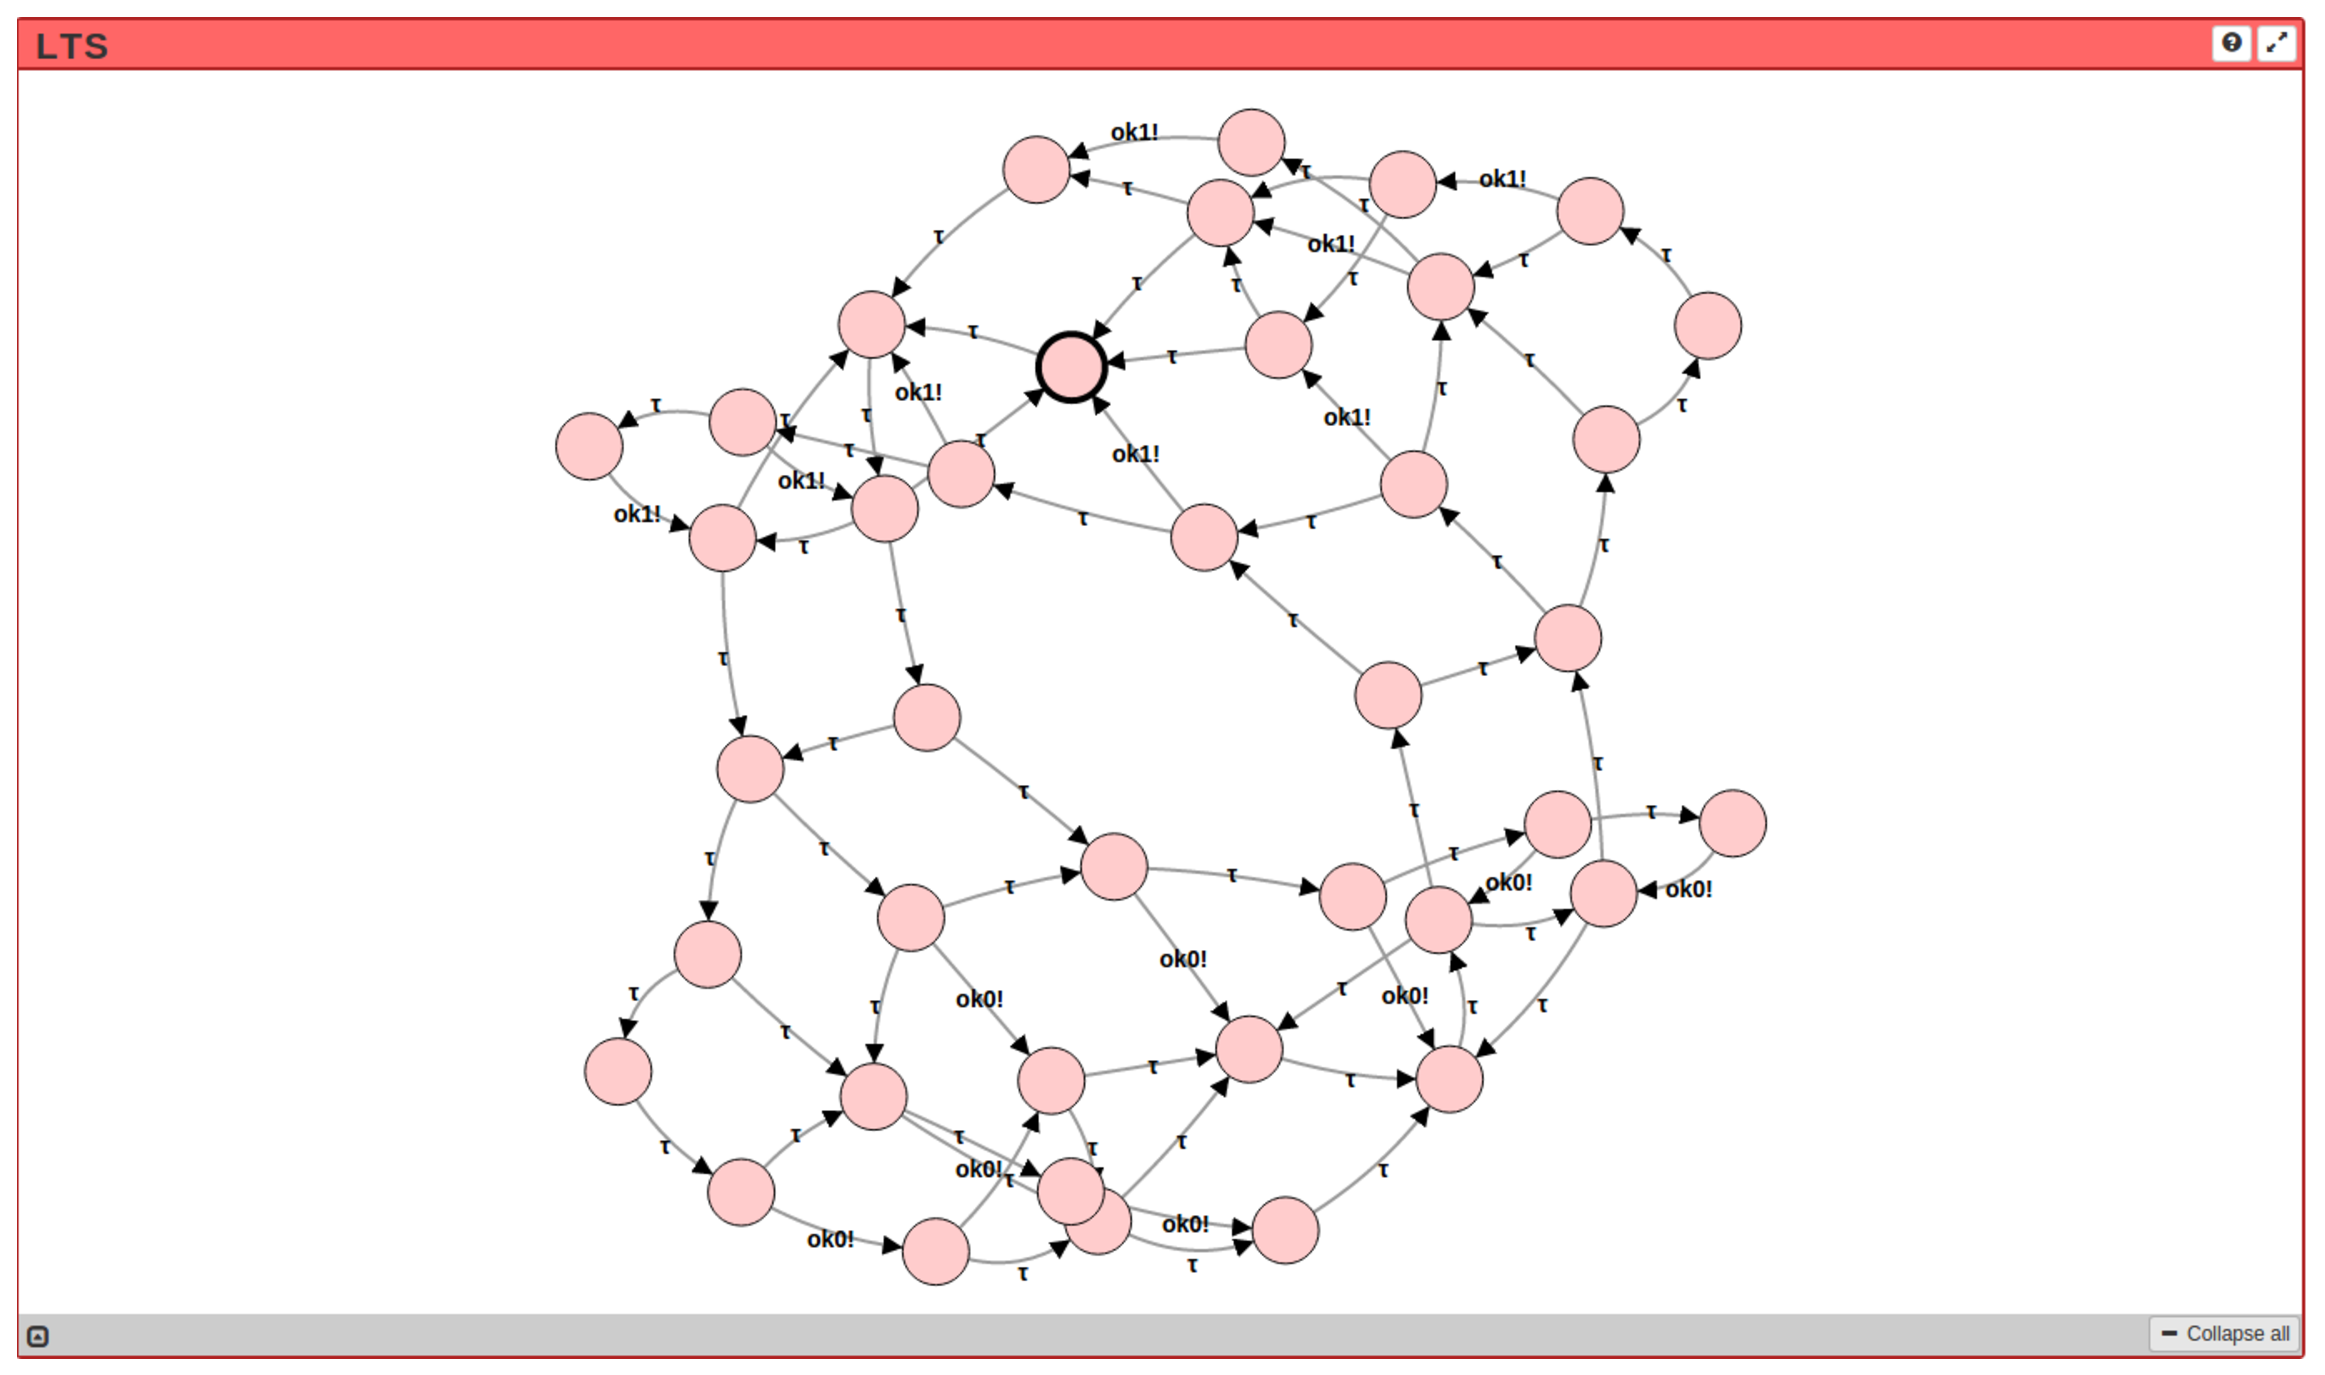
\includegraphics[width=.8\columnwidth]{images/pseuco.eps}
  \caption{\emph{LTS} disegnando da pseuCo}
  \label{fig:ccs-abp}
\end{figure}
 % 100%
\newpage{}\section{CWB}

\subsection{Utilizzo del WorkBench}

CWB (\emph{Concurrency WorkBench}) è uno strumento di analisi statica creato
per scopi accademici al fine di verificare diversi tipi di equivalenze e
proprietà.

Questo strumento è stato pensato principalmente per sistemi le cui
implementazioni sono definite con il CCS e forniscono la possibilità di
verificare delle proprietà espresse per mezzo della HML (\emph{Hennessy-Milner
Logic}).

Grazie alla successione di comandi presente in sezione \ref{sec:cwb-definition}
il workbench viene popolato con i sistemi visti in sezione
\ref{sec:ccs-model}.

Viene definita una specifica \textbf{Spec} tale che riesca a distinguere il
corretto alternarsi di messaggi con numero di sequenza 0 e 1:

$ > Spec = = ok_0.ok_1.Spec $

Vengono aggiunti anche due nuovi agenti e sistemi, distinguibili dal prefisso
\textbf{Loud}. In tali sistemi:

\begin{itemize}
  \item ogni volta che viene inviato un messaggio con numero di sequenza X
    da un \textbf{Sender}, viene effettuata una comunicazione sul canale
    \textbf{$send_X$};
  \item ogni volta che viene ricevuto un messaggio con numero di sequenza X
    da un \textbf{Receiver} o da un \textbf{BadReceiver}, viene effettuata una
    comunicazione sul canale \textbf{$receive_X$}.
\end{itemize}

\subsection{Verifica di proprietà}

A questo punto può essere utile vedere se il nostro sistema soddisfa delle
proprietà.

Per popolare il workbench e testare le proprietà desiderabili per questo,
vengono usati comandi estratti dal listato presente in sezione
\ref{sec:cwb-commands}.

\subsubsection{Presenza di deadlock}

Può essere utile sapere se i sistemi (sia quello affidabile che quello lossy)
possono andare in deadlock in qualche esecuzione. Dopo l'esecuzione del comando
\texttt{deadlocks(}$<Sys>$\texttt{)}, il workbench ci informa che non sono
presenti deadlock.

In questo caso il risultato rispecchia le attese, poichè:

\begin{enumerate}
  \item già in \textbf{pseuCo} si poteva notare che uno dei due sistemi non
    soffriva di deadlock;
  \item il protocollo in sè prevede che i messaggi vengano trasmessi
    continuamente, senza considerare situazioni in cui uno dei due nodi
    della rete si spegne o interruzioni di qualsiasi natura.
\end{enumerate}

\subsubsection{Bisimilarità forte}

Subito dopo essersi accertati dell'assenza di deadlock, è utile conoscere se i
sistemi individuati hanno un comportamento equivalente a quello della
specifica \textbf{Spec} ($Sys \sim Spec$).

Come è facile aspettarsi, nessuno dei due sistemi è fortemente bisimile alla
specifica. Tuttavia questo non stupisce, poichè nei due ABP vengono eseguite
delle azioni interne che la specifica non è capace di
eseguire\footnote{infatti con il comando
\texttt{dfstrong(}$<Sys>$\texttt{,Spec)} il workbench informa che il primo
``sa compiere'' un'azione interna \texttt{tau}}.

Nemmeno i due sistemi sono fortemente bisimili tra loro: il sistema lossy è
distinguibile a causa di una sequenza di azioni interne che prevede il rifiuto
del messaggio inviato. A causa di questo, non è vero che dopo cinque azioni
interne è sempre possibile vedere la comunicazione \texttt{$ok_0$}.

\subsubsection{Bisimilarità debole}

I due sistemi, però, ci si aspetta che siano debolmente bisimili alla
specifica poichè come visto prima l'unica differenza tra questi è la presenza
di azioni interne che permettono il corretto funzionamento del protocollo.

Dopo l'esecuzione dei comandi per tale verifica, il workbench conferma, come
aspettato, che i due sistemi e la specifica \textbf{Spec} precedentemente
definita sono debolmente bisimili.

\subsubsection{Proprietà HML}

Vengono verificate, sempre con l'ausilio dello stesso tool, un insieme di
proprietà per ogni sistema:

\paragraph{ReliableABP} \mbox{}

Per il sistema senza perdita di messaggi vengono provate le seguenti proprietà:

\begin{itemize}
  \item $Can(tau)$: vero -- il sistema può eseguire un'azione iniziale
    (interna)
  \item $Even(<ok_0>T)$: vero -- il sistema esegue sempre $ok_0$ in
    un'esecuzione completa
  \item $Even(<ok_1>T)$: vero -- il sistema esegue sempre $ok_1$ in
    un'esecuzione completa
  \item $Even([[ok_0]]<ok_1>T) \&{} Even([[ok_1]]<ok_0>T)$: vero -- in
    un'esecuzione completa, il sistema:
    \begin{itemize}
      \item per ogni modo in cui può eseguire $ok_0$, poi può eseguire $ok_1$;
      \item per ogni modo in cui può eseguire $ok_1$, poi può eseguire $ok_0$.
    \end{itemize}
  \item $Fair$: vero -- è invariante che in qualsiasi modo venga eseguito $ok$
    per un certo messaggio di sequenza, poi verrà eseguito quello per il
    messaggio con il numero di sequenza successivo;
  \item $Pos(<ok_0><ok_0>T | <ok_1><ok_1>T)$ falso -- viene testato che il
    \textbf{Receiver} non possa ricevere due messaggi consecutivi con lo stesso
    numero di sequenza;
  \item $NoConsecutiveSameNumber$ vero -- questa proprietà è la proprietà
    precedente negata;
  \item $Livelock$ falso -- non sono presenti Livelock nel presente, dal
    momento che non sono previsti \texttt{NACK} in questa implementazione.
\end{itemize}

\paragraph{UnreliableABP} \mbox{}

Per il sistema lossy vengono provate le seguenti proprietà:

\begin{itemize}
  \item $Even(<ok_0>T)$ falso -- non è vero che in tutte le computazioni
    complete venga ricevuto il messaggio con numero di sequenza 0, siccome il
    sistema potrebbe rimanere in ciclo infinito. \\
    In pratica, non vale la \emph{fair abstraction from divergence};
  \item $Even(<ok_1>T)$ falso -- non è vero che in tutte le computazioni
    complete venga ricevuto il messaggio con numero di sequenza 1, siccome il
    sistema potrebbe rimanere in ciclo infinito. \\
    In pratica, non vale la \emph{fair abstraction from divergence};
  \item $Fair$: vero -- è invariante che in qualsiasi modo venga eseguito $ok$
    per un certo messaggio di sequenza, poi verrà eseguito quello per il
    messaggio con il numero di sequenza successivo;
  \item $NoConsecutiveSameNumber$ vero -- il \textbf{BadReceiver} ignora i
    messaggi aventi numeri di sequenza uguali a quello ricevuto correttamente;
  \item $Livelock$ vero -- il \textbf{BadReceiver} potrebbe continuare aventi
    rifiutare un certo messaggio scegliendo di inviare sempre dei \texttt{NACK}
    all'\textbf{AckReceiver}.
\end{itemize}

\paragraph{LoudReliableABP} \mbox{}

Per l'implementazione estesa del protocollo con canale affidabile vengono
provate:

\begin{itemize}
  \item $LoudOk_0$ vero -- Ogniqualvolta un sistema manda un messaggio con
    numero di sequenza 0 (e dunque verrà effettuata una comunicazione sul
    canale $send_0$), questo verrà ricevuto (verrà effettuata una
    comunicazione sul canale $receive_0$);
  \item $LoudOk_1$ vero -- Ogniqualvolta un sistema manda un messaggio con
    numero di sequenza 1 (e dunque verrà effettuata una comunicazione sul
    canale $send_1$), questo verrà ricevuto (verrà effettuata una
    comunicazione sul canale $receive_1$);
  \item $LoudOk$ vero -- vero poichè entrambe le proprietà sopra descritte
    sono vere.
\end{itemize}

\paragraph{LoudUnreliableABP} \mbox{}

Per l'implementazione estesa del protocollo con canale affidabile vengono
provate:

\begin{itemize}
  \item $LoudOk_0$ falso -- Ogniqualvolta un sistema manda un messaggio con
    numero di sequenza 0 (e dunque verrà effettuata una comunicazione sul
    canale $send_0$), il canale ricevente potrebbe non accettarlo mai;
  \item $LoudOk_1$ falso -- Ogniqualvolta un sistema manda un messaggio con
    numero di sequenza 1 (e dunque verrà effettuata una comunicazione sul
    canale $send_1$), il canale ricevente potrebbe non accettarlo mai;
  \item $LoudOk$ falso -- falso poichè entrambe le proprietà sopra descritte
    sono false.
\end{itemize}
 % 0%
\newpage{}\section{Go}

\subsection{Perchè Go}\label{sec:why-do-we-go}

Google Go è un linguaggio di programmazione che basa i suoi principi sulla
gestione della concorrenza tramite comunicazione, mentre gran parte degli
altri linguaggi di programmazione utilizzano un approccio più vulnerabile,
condividendo memoria.

Condividendo canali di comunicazione, invece, è possibile realizzare programmi
robusti che riescano a soddisfare le stesse proprietà provate teoricamente con
strumenti come il CWB.

\subsection{Implementazione}

Il programma è stato implementato con le due versioni viste in precedenza,
ovvero quella che simula un canale affidabile (sez. \ref{sec:abp-prog}) e
quella che simula un canale con perdite (sez. \ref{sec:bad-abp-prog}).

I due programmi sono stati scritti tenendo conto che, come detto nella sezione
\ref{sec:why-do-we-go}, il paradigma pensato dai creatori di questo linguaggio
consisteva nel gestire la concorrenza tramite comunicazione e non condivisione
di memoria.

Questo ha permesso di riutilizzare gli script usati per definire gli agenti
usati nel CWB e trasformarli in pochissimo tempo in programmi equivalenti in
Go.

Ciascun agente è stato trasformato in una \emph{goroutine} e lanciate nel
metodo main, così come i canali condivisi vengono istanziati nel main e
passati esclusivamente a chi comunica su quei canali.
 % 0%

\appendix
\section{Programs}\label{sec:prog}

\subsection{abp.go}\label{sec:abp-prog}
\begin{verbatim}
\end{verbatim}

\subsection{abp\_bad.go}\label{sec:bad-abp-prog}
\begin{verbatim}
\end{verbatim}


%----------------------------------------------------------------------------------------

\newpage % Start the article content on the second page, remove this if you have a longer abstract that goes onto the second page

\end{document}
